\documentclass{article}

\usepackage{graphics}
\usepackage{epsfig}
\usepackage{color}
\usepackage[english]{babel}
\usepackage{graphicx}
\textwidth 6in
\addtolength{\oddsidemargin}{-0.5in}
\textheight 9in
\addtolength{\topmargin}{-0.5in}
\setlength{\parindent}{0pt}
\setlength{\parskip}{0.5cm}
\topskip 0.0in
\parindent 0.5in
\pagestyle{empty}
\thispagestyle{empty}
\title{\textbf{Onion Routing}\\
\large{Project Report : CS425 - Computer Networks}}

\author{Akshay Kumar\\
	Aman Sharma\\
	Chirag Gupta\\
	Deepak Pathak\\
	\\
	Advisor : Prof. Dheeraj Sanghi\\
        Department of Computer Science and Engineering\\
        IIT Kanpur
	}
%\date{Jan 1, 2012}
\date{\today}


\begin{document}
\maketitle

\begin{center}{ABSTRACT}
\end{center}
\textit{Onion Routing is a distributed P2P application that allows anonymous communication over computer network. Essentially speaking, in onion routing, messages are repeatedly encrypted and are then decrypted layer by layer by each of the nodes on its path. These nodes are termed as Onion Routers. This is analogous to onion peeling where each onion router uncovers a layer of encryption to discover a new routing instruction. It is also resistant to many security attacks such as denial of service attack, man in the middle attack, replay attack, etc and reliable against eavesdropping and sniffing. The mechanism of Onion Routing was originally developed by US Navy to send secure messages and is the backengine of the anonymous browser Tor.}

\section{Motivation}
Online anonymity is a very dificult problem which pressed the need for more secure and robust networks. In the worst case, attackers might have even access to all servers and be able to view all traffic passing in, through and out of the system. Hence, it is of utmost importance that system designers devise a security system which can encompass a wide range of hardware and be universal in nature. 

\section{Introduction to Onion Routing}
Onion routing is a way of providing secure communication on a P2P channel by using multiple layers of encryption. Instead of establishing a direct conection, the connection is routed via. multiple network nodes called onion routers. Every node has information only about its previous and next router's address. In this way, the router has no idea about the sender or the receiver of the data packet. It is assigned a key aproiri which it uses to decrypt one layer of encryption and then passes it on to next router without having gaining any knowledge about the contents of the message. In this way, only the last router has the real information about the contents of the message which it passes onto the destination.
\newline
\newline
The figure given below explains Onion Routing in a more concise way:
\begin{center}
 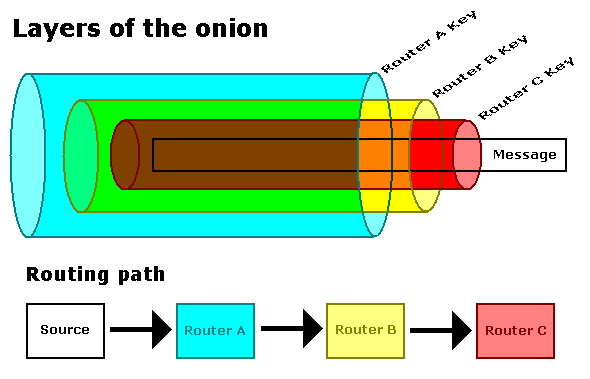
\includegraphics[scale=0.4]{Onion_diagram.png}
 \newline
 \small{Figure : Pictorial representation of Onion Routing}
 \newline
 \tiny{[Image Source : http://en.wikipedia.org/wiki/Onion\_routing]}
\end{center}

\section{Implementation Details}
We have designed a client, application proxy for the client, a set of n routers (here n=4) and a server for onion routing. Application proxy is a intermediary between client and routers which accepts message from client and encrypts it layer by layer and then passes it on to the router. The encrpytion is done in reverse order of the routers in such a way that the first key used to encrypt the message is of the router closest to the destination followed by the second closest router and so on.
\subsection*{AES Encryption}
Advanced Encryption Standard (AES) has been used for encrpytion. AES uses a symmetric key encrpytion, meaning that the same key is used both for encryption as well as decryption. Needless to say, each of the router is assigned a different key. Python contains a standard module Crpyto.Cipher which contains AES encrpytion and decryption functions.
\subsection*{Key Transfer}
At the onset of connection, right after the client, routers and server are up, the first thing application proxy does is to distribute the keys to each of the routers. First of all, the application proxy transmits the key to the first router in an unencrypted manner. Then for distributing the next key, it is first encrypted by key of the first router and is sent to the first router which decrypts it and forwards the actual key to the second router. In this way, every subsequent key is first encrypted through multiple levels of encryption and is then routed via previous routers.
\newline
\newline
Note that the key transmitted during setting up of connection contains both the AES Encryption Key and also the address of the next router. The address of the previous router is obtained trivially. In this way, every router has hold of only its previous and next router address. Also, so as to recognise that the intended data packet is a key transfer packet not a regular data packet, it is first padded by a starting delimiter.
\subsection*{Message Transfer}
Similar to key transfer protocol, the only difference in message transfer is that all the routers are now set up with their respective keys. It is to note that in our implementation, client waits for acknowledgement from server for certain amount of time and on timeout it resends the packet.
\newline
\newline
\begin{center}
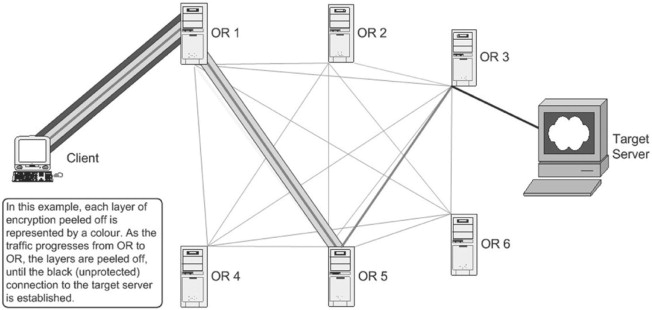
\includegraphics{onion.jpg}
\newline
 \small{Figure : Schematic representation of Onion Routing Network}
 \newline
 \tiny{[Image Source : http://www.sciencedirect.com/science/article/pii/S1353485807700442]}
 \newline
\end{center}
As evident from the figure shown above, the application level proxy is on the client machine. The client communicates to router via application proxy. The figure shows a message being sent from Client to OR1 encrypted multiple times. Each of the subsequent transmission strips off encrpytion by one level. Finally at the last router, the entire message gets decrypted and is forwarded to the destination.
\subsection*{Application Proxy}
Application Proxy does the network setting up on part of client and acts as interface between client and onion proxy provided constitutively by onion routers, giving client freedom of not knowing the actual protocol behind the scene. At the initialization time, the list of onion routers is available to it. It then decides an appropiate sequence of onion routers in order to transmit the message from the source to the destination. It distributes the keys to each of the routers. After this, network is set up. At the time of client to server communication, it encrypts the message whereas during server to client communication, it decrypts it and passes it to client.
\section{Conclusion and Future Scope}
Just like many other technologies, onion routing can be used for both positive and negative purposes. Criminals can evade identification in some cases using Onion Routing but this just can't be a reason for completely condemning onion routing. The users who are benefitting from onion routing right now are a pretty good reason for onion routing to continue. While it attracts it share of attackers, it continues to be the best tool for anonymity and free information access on the internet. It will be around for sometime to come.
\section{Acknowledgement}
We are highly indebted to express our sincerest gratitude to Prof. Dheeraj Sanghi without whose untiring help this project would not have been possible. He constant guidance throughout the course made the learning experience more enjoyful for us all. We are also very thankful to the TAs Vipin, Yogesh Kumar \& Abhishek Gera for their constant support and monitoring which helped us complete the project.
\section{References}
\begin{enumerate}
 \item Wikipedia \textit{Onion Routing} \texttt{http://en.wikipedia.org/wiki/Onion\_routing}
 \item Micheal Owen \textit{Fun with Onion Routing} \newline \texttt{http://www.sciencedirect.com/science/article/pii/S1353485807700442}
 \item Onion Routing \texttt{http://www.onion-router.net/}
 \item Wikipedia \textit{Advanced Encryption Standard} \newline \texttt{http://en.wikipedia.org/wiki/Advanced\_Encryption\_Standard}
\end{enumerate}

\end{document}